% Basiscursus Wiskunde - Lespakket 2
% Les 6. Gelijkheden - Ongelijkheden - Deelbaarheid
%
% Wijzigingen t.o.v. de originele bis-basis:
% * deze les voert de termen "eerste lid" en "tweede lid" in; wij gebruiken hier al
%   linkerlid en rechterlid, zoals in alle andere lessen (bv. les~16, les~31)
% * de Samenvatting aan het einde (vóór de oplossingen) is overgenomen uit het origineel; de
%   zin over vermenigvuldigen/delen bij een ongelijkheid is aangepast naar strikt positief/
%   strikt negatief, consistent met de correctie bij 6.2.2 hierboven
% * de oplossing van A.C.O. 2 verbindt de rekenstappen met <=> (via \LRA), zoals in de
%   andere lessen die vergelijkingen stap voor stap oplossen
% * de linkerlid/rechterlid/(on)gelijkheidsteken-schema's (6.1.1 en 6.2.1) zijn een klein
%   tikz-diagram met pijltjes naar de labels, i.p.v. de onderaccolades \underbrace die elders
%   worden gebruikt; dat blijft dichter bij de pijltjes in het origineel en houdt het
%   ongelijkheidsschema smal
% * bij 6.2.2, eigenschap 2) vermeldt het origineel enkel het vermenigvuldigen/delen met een
%   positief getal (in tekst en voorbeelden); het Besluit veralgemeent dat foutief naar "een
%   nieuwe ongelijkheid in dezelfde zin" voor elk van nul verschillend getal. Toegevoegd: een
%   voorbeeld met een strikt negatief getal (het teken draait om) en het genuanceerde Besluit
%   (strikt positief: dezelfde zin, strikt negatief: tegengestelde zin); "strikt" om duidelijk
%   te maken dat nul niet meetelt
% * bij 6.2.2, eigenschap 3) geldt kwadrateren/vierkantswortel trekken enkel als beide leden
%   niet-negatief zijn (het origineel vermeldt die voorwaarde niet); toegevoegd: die voorwaarde
%   in het Besluit en een tegenvoorbeeld met twee negatieve getallen waarbij kwadrateren de
%   ongelijkheid omdraait
% * A.C.O. 11: "<deler>: <getal>" vermeden, want de dubbele punt oogt in dit hoofdstuk als een
%   deling; elk item is nu "<getal> deelbaar door <deler>"
% * bij 6.4.2 staat de uitleg bij de eerste praktische schikking (108) in een minipage naast de
%   tabel i.p.v. eronder, zoals in het origineel, waar de tekst naast elke regel van de deling
%   staat
% * de praktische schikking (het "getal | priemfactor"-tabelletje) komt tientallen keren voor in
%   6.4; i.p.v. elke tabel en haar ontbinding met de hand te schrijven, berekenen de macro's
%   \priemfactorisatie{<n>}/\priemontbind[h|v]{<n>} (preambule) de priemontbinding van <n> zelf
%   (staartdeling in TeX-rekenregisters) en zetten ze de tabel en/of de machtsnotatie op; enkel
%   het getal zelf staat dus nog in de brontekst. Geverifieerd tegen alle 15 tabellen uit het
%   origineel vóór het invoegen. Kleine bijwerking: 2\,365 wordt hierdoor zonder dunne spatie als
%   2365 weergegeven (de macro kent geen duizendtalgroepering)
%
% Openstaande opmerkingen:
% *

\documentclass{bis}

% Voor het pijltje van "2^3" naar de toelichtende zin in 6.4.3 (kgv(24,60)-voorbeeld): laat
% opeenvolgende nodes automatisch tegen elkaar aansluiten zonder de breedtes met de hand te
% moeten opmeten.
\usetikzlibrary{positioning}

% \priemfactorisatie{<n>}: enkel "<n>=<ontbinding>", voor wanneer de tabel al elders staat.
% \priemontbind[h|v]{<n>}: tabel en "<n>=<ontbinding>" samen; h (standaard) naast elkaar, v
% erboven/eronder. Aan de hand van het getal alleen: de macro deelt zelf herhaald door het
% kleinst mogelijke priemgetal (staartdeling in TeX-rekenregisters, geen pgfmath, om
% afrondingsfouten bij grotere getallen te vermijden) en bouwt zowel de tabel
% als de machtsnotatie op.
\makeatletter
\newcount\priem@n
\newcount\priem@p
\newcount\priem@mod
\newcount\priem@tmp
\newcount\priem@curp
\newcount\priem@curexp
\newif\ifpriem@first

\newcommand{\priem@compute}[1]{%
  \def\priem@rows{}%
  \def\priem@prod{}%
  \priem@curp=0
  \priem@curexp=0
  \priem@firsttrue
  \priem@n=#1\relax
  \priem@p=2\relax
  \priem@loop
}

\def\priem@loop{%
  \ifnum\priem@n=1
    \priem@addrow{1}{}%
    \priem@flush
  \else
    \priem@tmp=\priem@n
    \divide\priem@tmp by\priem@p
    \multiply\priem@tmp by\priem@p
    \priem@mod=\priem@n
    \advance\priem@mod by-\priem@tmp
    \ifnum\priem@mod=0
      \priem@addrow{\the\priem@n}{\the\priem@p}%
      \ifnum\priem@p=\priem@curp
        \advance\priem@curexp by1
      \else
        \priem@flush
        \priem@curp=\priem@p
        \priem@curexp=1
      \fi
      \divide\priem@n by\priem@p
      \priem@loop
    \else
      \advance\priem@p by1
      \priem@loop
    \fi
  \fi
}

\newcommand{\priem@addrow}[2]{%
  \ifpriem@first
    \priem@firstfalse
    \edef\priem@rows{#1 & #2}%
  \else
    \edef\priem@rows{\priem@rows\noexpand\\#1 & #2}%
  \fi
}

\newcommand{\priem@flush}{%
  \ifnum\priem@curp=0
  \else
    \ifnum\priem@curexp=1
      \edef\priem@thisterm{\the\priem@curp}%
    \else
      \edef\priem@thisterm{\the\priem@curp^{\the\priem@curexp}}%
    \fi
    \ifx\priem@prod\empty
      \edef\priem@prod{\priem@thisterm}%
    \else
      \edef\priem@prod{\priem@prod\noexpand\cdot\priem@thisterm}%
    \fi
  \fi
}

\newcommand{\priemfactorisatie}[1]{\begingroup\priem@compute{#1}#1=\priem@prod\endgroup}
% \priemontbind[h]{<n>} (standaard): tabel en "<n>=<ontbinding>" naast elkaar.
% \priemontbind[v]{<n>}: tabel erboven, resultaat eronder; het resultaat staat op de onderste
% rij van een [b]-array, zodat meerdere \priemontbind[v]-blokken naast elkaar hun resultaatregel
% op dezelfde hoogte houden, ook als de tabellen zelf een verschillend aantal rijen hebben.
\newcommand{\priemontbind}[2][h]{%
  \begingroup
  \priem@compute{#2}%
  \ifthenelse{\equal{#1}{v}}
    {\begin{array}[b]{c}\begin{array}{r|l}\priem@rows\end{array}\\[1em]#2=\priem@prod\end{array}}
    {\begin{array}{r|l}\priem@rows\end{array}\qquad#2=\priem@prod}%
  \endgroup
}
\makeatother

\begin{document}

\les{6}{Gelijkheden - Ongelijkheden - Deelbaarheid}

\subsection{Gelijkheden}

\subsubsection{Begrip}

\[3+2=5\qquad\text{Deze ware uitspraak noemt men een \emph{gelijkheid}.}\]
Een gelijkheid bestaat uit 2 delen:
\begin{itemize}
  \item het deel voor het gelijkheidsteken is het \textbf{linkerlid};
  \item het deel na het gelijkheidsteken is het \textbf{rechterlid}.
\end{itemize}
\begin{center}
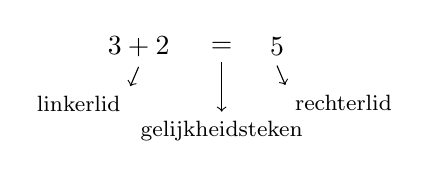
\begin{tikzpicture}[x=1em,y=1em]
\node (a) at (0,0) {$3+2$};
\node (b) at (3,0) {$=$};
\node (c) at (5,0) {$5$};
\draw[->] (a.south) -- ++(-0.3,-0.7) node[below left] {\footnotesize linkerlid};
\draw[->] (b.south) -- ++(0,-1.8) node[below] {\footnotesize gelijkheidsteken};
\draw[->] (c.south) -- ++(0.3,-0.7) node[below right] {\footnotesize rechterlid};
\end{tikzpicture}
\end{center}

\subsubsection{Eigenschappen}

\subsubsection*{Optellen en aftrekken.}
We tellen bij beide leden van de gelijkheid $3+2=5$ eenzelfde getal op, bijvoorbeeld 6:
\[(3+2)+6=5+6.\]
We bekomen een nieuwe gelijkheid. Tellen we bij beide leden 17 op, dan bekomen we ook een
gelijkheid:
\[(3+2)+17=5+17.\]
We trekken van beide leden 3 af:
\[(3+2)-3=5-3.\]
Ook in dit geval ontstaat er een nieuwe gelijkheid.
\begin{onthoud}
Als men bij beide leden van een gelijkheid eenzelfde getal optelt of eenzelfde getal aftrekt,
bekomt men een nieuwe gelijkheid.
\end{onthoud}

\subsubsection*{Vermenigvuldigen en delen.}
We controleren of deze eigenschap ook geldt als we beide leden vermenigvuldigen met of delen
door eenzelfde getal.
\[8+4=15-3\qquad\text{Dit is een gelijkheid.}\]
We vermenigvuldigen elk lid met 2:
\[(8+4)\cdot2=(15-3)\cdot2.\]
We bekomen een nieuwe gelijkheid. Deel nu elk lid door 4:
\[(8+4):4=(15-3):4.\]
We bekomen opnieuw een gelijkheid. Let op: dit geldt niet als je door nul deelt.
\begin{onthoud}
Als men beide leden van een gelijkheid vermenigvuldigt met of deelt door eenzelfde getal,
bekomt men een nieuwe gelijkheid.
\end{onthoud}

\subsubsection*{Machtsverheffen en vierkantswortel trekken.}
Deze eigenschap geldt ook bij machtsverheffing en vierkantsworteltrekking.
\[18-15=3\quad\Rightarrow\quad(18-15)^2=3^2\]
en ook
\[16-7=5+4\quad\Rightarrow\quad\sqrt{16-7}=\sqrt{5+4}.\]
$\Rightarrow$ lees je als \emph{'daaruit volgt'} of \emph{'als \dots\ dan \dots'}. Men noemt deze
pijl de \textbf{implicatiepijl}.
\begin{onthoud}
Als men beide leden van een gelijkheid tot een macht verheft, of uit beide leden de
vierkantswortel trekt, bekomt men een nieuwe gelijkheid.
\end{onthoud}

\begin{exercise}
Vul aan, gebruik bovenvermelde eigenschappen.
\begin{enumerate}
  \item Als $a+3=b+2$ dan $a+1=\ldots$
  \item Als $a+8=b-2$ dan $a-2=\ldots$
  \item $8+a=7-b\ \Rightarrow\ (8+a)^3=\ldots$
  \item $a+5=b+3\ \Rightarrow\ 2a+10=\ldots$
\end{enumerate}
\end{exercise}

\begin{solution}
\begin{enumerate}
  \item $a+1=b$
  \item $a-2=b-12$
  \item $(8+a)^3=(7-b)^3$
  \item $2a+10=2b+6$
\end{enumerate}
\end{solution}

\subsubsection{Eigenschappen van 2 of meer gelijkheden}

\[5+7=12\quad\text{en}\quad6=8-2\]
Als we bij beide leden hetzelfde getal optellen, hebben we opnieuw een gelijkheid:
\[5+7+6=12+6.\]
Uit de 2de gelijkheid blijkt dat $6=8-2$. In het rechterlid van de 1ste gelijkheid vervangen we
6 door $8-2$:
\[5+7+6=12+(8-2).\]
Op deze manier is het linkerlid van de 1ste gelijkheid opgeteld bij het linkerlid van de 2de
gelijkheid, en ook het rechterlid van de 1ste gelijkheid bij het rechterlid van de 2de
gelijkheid. Men zegt: deze gelijkheden zijn \emph{lid aan lid opgeteld}.

Ook geldt dat:
\begin{align*}
(5+7)-6&=12-(8-2)\\
(5+7)\times6&=12\times(8-2)\\
(5+7):6&=12:(8-2)
\end{align*}
\begin{onthoud}
Als men 2 gegeven gelijkheden lid aan lid optelt, aftrekt, vermenigvuldigt of deelt, dan bekomt
men een nieuwe gelijkheid.
\end{onthoud}

\begin{exercise}
Gegeven: $a^2+b^2=202$ en $a^2-b^2=40$.
\begin{enumerate}
  \item Tel beide gelijkheden lid aan lid op en bereken hieruit de waarde van $a$.
  \item Trek beide gelijkheden lid aan lid af en bereken hieruit de waarde van $b$.
\end{enumerate}
\end{exercise}

\begin{solution}
\begin{enumerate}
  \item
  \begin{alignat*}{2}
       &&a^2+b^2+a^2-b^2&=202+40\\
  \LRA &&2a^2&=242\\
  \LRA &&a^2&=121\\
  \LRA &&a&=11
  \end{alignat*}
  \item
  \begin{alignat*}{2}
       &&a^2+b^2-(a^2-b^2)&=202-40\\
  \LRA &&a^2+b^2-a^2+b^2&=162\\
  \LRA &&2b^2&=162\\
  \LRA &&b^2&=81\\
  \LRA &&b&=9
  \end{alignat*}
\end{enumerate}
\end{solution}

\subsubsection{Transitieve eigenschap}

\[8-3=5\qquad\text{en}\qquad5=1+4\qquad\text{dan}\qquad8-3=1+4.\]
\[a=b\text{ en }b=c\quad\Rightarrow\quad a=c\]
\begin{onthoud}
Als 2 getallen gelijk zijn aan eenzelfde derde getal, dan zijn deze 2 getallen ook aan elkaar
gelijk.
\end{onthoud}
Deze eigenschap noemt men de \textbf{transitiviteit} van de gelijkheid.

\begin{exercise}
Schrijf volgende gelijkheden met symbolen.
\begin{enumerate}
  \item de som van $a$ en $b$ is gelijk aan 7
  \item het verschil van $c$ en $d$ is gelijk aan 10
  \item de som van $e$ en $f$ is gelijk aan het verschil van $x$ en $y$
  \item het getal $a$ is 5 meer dan $b$
  \item het getal $c$ is 7 minder dan $d$
  \item trekt men van 20 het getal $x$ af, dan bekomt men de som van $m$ en $n$
  \item het product van $k$ met $l$ is 12
  \item het quotiënt van $a$ en $b$ is gelijk aan 15
  \item het product van $c$ met $d$ is 4 meer dan het verschil van $x$ en $y$
  \item het getal $k$ is 7 minder dan het quotiënt van $m$ en 4
\end{enumerate}
\end{exercise}

\begin{solution}
\begin{enumerate}
  \item $a+b=7$
  \item $c-d=10$
  \item $e+f=x-y$
  \item $a-5=b$ of $a=b+5$
  \item $c+7=d$ of $c=d-7$
  \item $20-x=m+n$
  \item $k\cdot l=12$
  \item $a:b=15$
  \item $c\cdot d-4=x-y$ of $c\cdot d=x-y+4$
  \item $k+7=m:4$ of $k=m:4-7$
\end{enumerate}
\end{solution}

\begin{exercise}
Gegeven: $a-b=c+d$. Als $a,b,c,d$ dezelfde waarde hebben als in het gegeven, welke onderstaande
uitdrukking is dan juist?
\begin{meerkeuze}
  \item $a-c=d-b$
  \item $b=c+d-a$
  \item $a-d=c+b$
  \item $c+d+a=b$
\end{meerkeuze}
\end{exercise}

\begin{solution}
\textbf{Antwoord (C)} is juist.
\end{solution}

\subsection{Ongelijkheden}

\subsubsection{Begrip}

\begin{center}
\begin{tabular}{ll}
$5\neq3$ & 5 is niet gelijk aan 3 of 5 is verschillend van 3\\
$5>3$ & 5 is groter dan 3\\
$5\geq3$ & 5 is groter dan of gelijk aan 3\\
$3<5$ & 3 is kleiner dan 5\\
$3\leq5$ & 3 is kleiner dan of gelijk aan 5
\end{tabular}
\end{center}
Ook bij een ongelijkheid onderscheiden we 2 delen:
\begin{center}
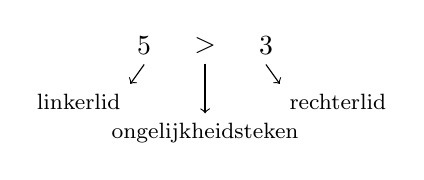
\begin{tikzpicture}[x=1em,y=1em]
\node (a) at (0,0) {$5$};
\node (b) at (2.2,0) {$>$};
\node (c) at (4.4,0) {$3$};
\draw[->] (a.south) -- ++(-0.5,-0.7) node[below left] {\footnotesize linkerlid};
\draw[->] (b.south) -- ++(0,-1.8) node[below] {\footnotesize ongelijkheidsteken};
\draw[->] (c.south) -- ++(0.5,-0.7) node[below right] {\footnotesize rechterlid};
\end{tikzpicture}
\end{center}

\begin{exercise}
Welke gehele waarden kan $a$ aannemen in volgende ongelijkheden?
\begin{enumerate}
  \item $a<7$
  \item $2<a<6$
  \item $5\leq a$
  \item $a>10$
  \item $7\leq a<9$
\end{enumerate}
\end{exercise}

\begin{solution}
\begin{enumerate}
  \item $0,1,2,3,4,5,6$
  \item $3,4,5$
  \item $5,6,7,\ldots$
  \item $11,12,13,\ldots$
  \item $7,8$
\end{enumerate}
\end{solution}

\subsubsection{Eigenschappen}

\subsubsection*{1) Beide leden van een ongelijkheid vermeerderen of verminderen met eenzelfde getal.}
\[12>10\]
We tellen bij beide leden van deze ongelijkheid eenzelfde getal op, bijvoorbeeld 10:
\[12+10>10+10\qquad\text{of}\qquad22>20.\]
We trekken nu van beide leden eenzelfde getal af:
\[12-6>10-6\qquad\text{of}\qquad6>4.\]
Het teken '$>$' blijft behouden als we bij beide leden eenzelfde getal optellen of aftrekken. We
zeggen: we bekomen een nieuwe ongelijkheid \emph{in dezelfde zin}. We controleren dit ook voor
een ander ongelijkheidsteken:
\[16<20\qquad\text{en ook}\qquad16+3<20+3.\]
\begin{onthoud}
Als men bij beide leden van een ongelijkheid eenzelfde getal optelt of eenzelfde getal aftrekt,
bekomt men een nieuwe ongelijkheid in dezelfde zin.
\end{onthoud}

\textit{Gevolg}

\begin{voorbeeld}
$10+3>11$. We trekken van beide leden 3 af:
\[10>11-3.\]
Merk op dat niet alleen de term $+3$ van lid verandert, maar dat ook het bijbehorend teken
wijzigt: $+3$ in het linkerlid wordt $-3$ in het rechterlid.
\end{voorbeeld}

\begin{voorbeeld}
$8-2<12$. We tellen bij beide leden 2 op:
\[8<12+2.\]
De term 2 is veranderd van lid, maar ook het teken is veranderd: $-2$ in het linkerlid is $+2$
in het rechterlid.
\end{voorbeeld}

\begin{onthoud}
In een ongelijkheid mogen we een term van lid veranderen, op voorwaarde dat we ook zijn teken
veranderen.
\end{onthoud}

\begin{exercise}
\begin{enumerate}
  \item $a+b-5<10\ \Rightarrow\ a+b<\ldots$
  \item $a-3+c\leq b\ \Rightarrow\ -3+c\leq\ldots$
  \item $a>4-b\ \Rightarrow\ b>\ldots$
\end{enumerate}
\end{exercise}

\begin{solution}
\begin{enumerate}
  \item $a+b<15$
  \item $-3+c\leq b-a$
  \item $b>4-a$
\end{enumerate}
\end{solution}

\subsubsection*{2) Beide leden van een ongelijkheid vermenigvuldigen met of delen door eenzelfde getal.}
\[12>10\]
We vermenigvuldigen beide leden met eenzelfde getal:
\[12\cdot2>10\cdot2\qquad\text{of}\qquad24>20.\]
Er ontstaat een nieuwe ongelijkheid in dezelfde zin. Dit geldt echter niet als we beide leden
vermenigvuldigen met nul:
\[12\cdot0=10\cdot0.\]
We delen beide leden door 2:
\[12:2>10:2\qquad\text{of}\qquad6>5.\]
Er ontstaat opnieuw een ongelijkheid in dezelfde zin.

We vermenigvuldigen nu beide leden met een \emph{strikt negatief} getal, bijvoorbeeld $-2$:
\[12\cdot(-2)=-24\qquad\text{en}\qquad10\cdot(-2)=-20.\]
Vergelijk: $-24<-20$, terwijl $12>10$. Het ongelijkheidsteken is dus \textbf{omgedraaid}: we
bekomen een nieuwe ongelijkheid in de \emph{tegengestelde} zin.

\textbf{Opgelet.} Delen door 0 is onmogelijk (of zinledig).
\begin{onthoud}
Als men beide leden van een ongelijkheid vermenigvuldigt met of deelt door eenzelfde
\emph{strikt positief} getal, bekomt men een nieuwe ongelijkheid in dezelfde zin. Vermenigvuldigt
of deelt men met eenzelfde \emph{strikt negatief} getal, dan bekomt men een nieuwe ongelijkheid
in de \emph{tegengestelde} zin: het ongelijkheidsteken draait om.
\end{onthoud}

\subsubsection*{3) Van beide leden van een ongelijkheid het kwadraat of de vierkantswortel bepalen.}
\[12>10\]
We verheffen beide leden tot de 2de macht:
\[12^2>10^2\qquad\text{of}\qquad144>100.\]
\[9<16\]
We trekken van beide leden de vierkantswortel:
\[\sqrt9<\sqrt{16}\qquad\text{of}\qquad3<4.\]

Dit mag enkel als beide leden \emph{niet-negatief} zijn: de vierkantswortel van een negatief
getal bestaat niet, en bij het kwadrateren van twee negatieve getallen draait de ongelijkheid
net om. Bijvoorbeeld:
\[-10>-12\qquad\text{maar}\qquad(-10)^2=100<144=(-12)^2.\]
\begin{onthoud}
Als men beide leden van een ongelijkheid, die \emph{niet-negatief} zijn, tot een macht verheft,
of uit beide leden de vierkantswortel trekt, bekomt men een nieuwe ongelijkheid in dezelfde zin.
\end{onthoud}

\begin{exercise}
Vul aan en noteer welke gehele waarden $a$ kan aannemen in volgende gevallen.
\begin{enumerate}
  \item $4a<20\ \Rightarrow\ a<\ldots$
  \item $a^2\geq25\ \Rightarrow\ a\ \ldots$
\end{enumerate}
\end{exercise}

\begin{solution}
\begin{enumerate}
  \item $a<5$: $a$ kan zijn $0,1,2,3,4$
  \item $a\geq5$: $5,6,7,\ldots$
\end{enumerate}
\end{solution}

\subsubsection*{4) Eigenschappen van 2 of meer ongelijkheden.}
Indien men 2 ongelijkheden heeft in dezelfde zin,
\[5>4\qquad\text{en}\qquad9>6,\]
dan bekomt men een nieuwe ongelijkheid in dezelfde zin als men beide ongelijkheden lid aan lid
optelt,
\[5+9>4+6\qquad\text{of}\qquad14>10,\]
of lid aan lid vermenigvuldigt:
\[5\cdot9>4\cdot6\qquad\text{of}\qquad45>24.\]

Deze eigenschap geldt echter niet voor aftrekken en delen. We illustreren dit door middel van
enkele voorbeelden.
\[
\begin{array}{ccc}
8>4\text{ en }5>3 & 8>7\text{ en }5>3 & 8>7\text{ en }5>4\\
8-5>4-3 & 8-5<7-3 & 8-5=7-4\\
3>1 & 3<4 & 3=3
\end{array}
\]
\[
\begin{array}{ccc}
8>4\text{ en }4>2 & 8>6\text{ en }4>2 & 8>3\text{ en }2>1\\
8:4=4:2 & 8:4<6:2 & 8:2>3:1\\
2=2 & 2<3 & 4>2
\end{array}
\]
Indien men 2 ongelijkheden in dezelfde zin lid aan lid aftrekt of deelt, bekomt men een
ongelijkheid in dezelfde zin, in tegengestelde zin, of zelfs een gelijkheid.
\begin{onthoud}
Indien men 2 ongelijkheden in dezelfde zin lid aan lid optelt of vermenigvuldigt, bekomt men een
nieuwe ongelijkheid in dezelfde zin.
\end{onthoud}

\subsubsection*{5) Transitieve eigenschap.}
\[5>3\text{ en }3>1\text{ dan }5>1\qquad\qquad10<15\text{ en }15<20\text{ dan }10<20\]
\begin{onthoud}
\begin{align*}
a>b\text{ en }b>c&\quad\Rightarrow\quad a>c\\
a<b\text{ en }b<c&\quad\Rightarrow\quad a<c
\end{align*}
\end{onthoud}

\subsubsection*{6) Aftrekken van ongelijkheden in tegengestelde zin.}
\[8>5\qquad\text{en}\qquad2<3\]
We trekken deze ongelijkheden lid aan lid af:
\[8-2>5-3\qquad\text{of}\qquad6>2.\]
We bekomen een nieuwe ongelijkheid in dezelfde zin als de eerste.
\begin{onthoud}
\[a>b\text{ en }c<d\quad\Rightarrow\quad a-c>b-d\]
\end{onthoud}
\textbf{Bewijs.} We plaatsen de ongelijkheden in dezelfde zin onder elkaar en tellen lid aan lid
op.
\[
\begin{array}{r@{\ }c@{\ }l@{\qquad}c@{\qquad}r@{\ }c@{\ }l@{\quad}l}
a&>&b & & a&>&b &\\
c&<&d &\Rightarrow& +\qquad d&>&c &\text{ongelijkheid in dezelfde zin}\\
\cline{5-7}
& & & & a+d&>&b+c &\text{lid aan lid optellen}\to\text{ongelijkheid in dezelfde zin}\\
& & &\Leftrightarrow&a-c&>&b-d &\text{verwissel $c$ en $d$ van lid}
\end{array}
\]

\begin{exercise}
Gegeven: $a+b<c+d$. In welke uitdrukking is het ongelijkheidsteken juist?
\begin{meerkeuze}
  \item $c+d+3<a+b+3$
  \item $(a-d)^2>(c-b)^2$
  \item $c-a+d-b<0$
  \item $2a-2c<2d-2b$
\end{meerkeuze}
\end{exercise}

\begin{solution}
\textbf{Antwoord (D)}: $b$ en $c$ verwisselen van lid; daarna worden beide leden $\times2$.
\end{solution}

\subsection{Deelbaarheid}

\subsubsection{Begrippen}

Als je een getal vermenigvuldigt met 6, dan bekom je een veelvoud van 6.
\[5\cdot6=30\qquad8\cdot6=48\]
30 en 48 zijn \emph{veelvouden} van 6, of: 6 is een \emph{deler} van 30, of: 30 is
\emph{deelbaar} door 6.

6 is een deler van 30, dan is $30:6$ een \emph{opgaande deling}, of m.a.w. de rest van de deling
is 0.

\subsubsection{Kenmerken van deelbaarheid}

Voor sommige getallen kan je op een eenvoudige wijze controleren of ze een deler zijn van een
bepaald getal. Dit noemen we de \textbf{kenmerken van deelbaarheid}.

\subsubsection*{1) Deelbaarheid door 2, 5, 10.}
Een getal is deelbaar door 2, 5 of 10 als het laatste cijfer van het getal deelbaar is door
respectievelijk 2, 5 of 10.
\begin{itemize}
  \item Een getal is deelbaar door 2 als het eindigt op 0, 2, 4, 6 of 8. Voorbeelden: 128,
  6\,280, 15\,824 zijn deelbaar door 2.
  \item Een getal is deelbaar door 5 als het getal eindigt op 0 of 5. Voorbeelden: 125,
  125\,840, 220 zijn deelbaar door 5.
  \item Een getal is deelbaar door 10 als het eindigt op 0.
\end{itemize}

\subsubsection*{2) Deelbaarheid door 4, 25 en 100.}
Een getal is deelbaar door 4, 25 of 100 als de laatste 2 cijfers deelbaar zijn door
respectievelijk 4, 25 of 100.
\begin{itemize}
  \item Een getal is deelbaar door 100 als de laatste 2 cijfers nullen zijn. Voorbeelden:
  1\,000, 22\,500, 800 zijn deelbaar door 100.
  \item Een getal is deelbaar door 4 als het getal gevormd door de laatste 2 cijfers deelbaar is
  door 4. Voorbeeld: 1\,248 is deelbaar door 4 want 48 is deelbaar door 4.
  \item Een getal is deelbaar door 25 als het eindigt op 00, 25, 50 of 75. Voorbeelden: 175,
  3\,825, 2\,050 zijn veelvouden van 25.
\end{itemize}

\subsubsection*{3) Deelbaarheid door 3 en 9.}
\begin{itemize}
  \item Een getal is deelbaar door 3 als de som van de cijfers van dat getal deelbaar is door 3.
  Voorbeeld: 92\,871 is deelbaar door 3 want $9+2+8+7+1=27$ en 27 is een veelvoud van 3.
  \item Een getal is deelbaar door 9 als de som van de cijfers deelbaar is door 9. Voorbeeld:
  1\,233 is deelbaar door 9 want $1+2+3+3=9$ en 9 is deelbaar door 9.
\end{itemize}

\subsubsection*{4) Deelbaarheid door 8, 125 en 1\,000.}
\begin{itemize}
  \item Een getal is deelbaar door 8 als het getal gevormd door de laatste 3 cijfers deelbaar is
  door 8. Voorbeeld: 1\,216 is deelbaar door 8, want 216 is deelbaar door 8.
  \item Een getal is deelbaar door 125 als de laatste 3 cijfers 000, 125, 250, 375, 500, 625,
  750 of 875 zijn. Voorbeeld: 1\,250, 11\,625, 9\,875 zijn deelbaar door 125.
  \item Een getal is deelbaar door 1\,000 als het eindigt op 000. Voorbeeld: 8\,000, 165\,000
  zijn deelbaar door 1\,000.
\end{itemize}

\subsubsection*{5) Deelbaarheid door 11.}
Een getal is deelbaar door 11 als het verschil van de som van de cijfers van de oneven rangen en
de som van de cijfers van de even rangen deelbaar is door 11.

\begin{voorbeeld}
4\,928. We nummeren de rangen van rechts naar links (4de, 3de, 2de, 1ste).\\
Som van de cijfers van oneven rang: $8+9=17$.\\
Som van de cijfers van even rang: $2+4=6$.\\
Verschil: $17-6=11$. 11 is een veelvoud van 11, dus 4\,928 is een veelvoud van 11.
\end{voorbeeld}

\begin{voorbeeld}
181\,929.\\
Som van de cijfers van oneven rang: $9+9+8=26$.\\
Som van de cijfers van even rang: $2+1+1=4$.\\
Verschil: $26-4=22$. 181\,929 is deelbaar door 11 want 22 is deelbaar door 11.
\end{voorbeeld}

\begin{voorbeeld}
9\,152.\\
Som van de cijfers van oneven rang: $2+1=3$.\\
Som van de cijfers van even rang: $5+9=14$.\\
Verschil: $3-14=?$ Indien de aftrekker groter is dan het aftrektal, vermeerderen we het
aftrektal met 11: $14-14=0$.\\
9\,152 is deelbaar door 11, want $0:11=0$.
\end{voorbeeld}

\begin{exercise}
$6\,470,\ 2\,854,\ 9\,185,\ 276,\ 1\,404,\ 82\,100$.\\
Onderzoek welke bovenstaande getallen deelbaar zijn:
\begin{multicols}{3}
\begin{enumerate}
  \item door 2
  \item door 3
  \item door 4
  \item door 8
  \item door 9
  \item door 10
  \item door 100
  \item door 11
  \item door 125
\end{enumerate}
\end{multicols}
\end{exercise}

\begin{solution}
\begin{enumerate}
  \item door 2: $6\,470,\ 2\,854,\ 276,\ 1\,404,\ 82\,100$
  \item door 3: $276,\ 1\,404$
  \item door 4: $276,\ 1\,404,\ 82\,100$
  \item door 8: geen
  \item door 9: $1\,404$
  \item door 10: $6\,470,\ 82\,100$
  \item door 100: $82\,100$
  \item door 11: $9\,185$
  \item door 125: geen
\end{enumerate}
\end{solution}

\begin{exercise}
Controleer of volgende getallen 11-vouden zijn. Vervang in de getallen die geen 11-voud zijn, de
nullen door een beduidend cijfer, zodat er een 11-voud ontstaat.
\[8\,059,\quad232\,034,\quad28\,130,\quad11\,079\]
\end{exercise}

\begin{solution}
\begin{itemize}
  \item $8\,059$: som oneven rangen $-$ som even rangen $=(9+11)-13=7$. 7 is geen elfvoud, dus
  8\,059 ook niet. Wel elfvoud: 8\,459.
  \item $232\,034$: verschil $7-7=0$, is een elfvoud.
  \item $28\,130$: verschil $(3+11)-11=3$, geen elfvoud. Wel elfvoud: 28\,138.
  \item $11\,079$: verschil $10-8=2$, geen elfvoud. 11\,979 wel elfvoud, want $19-8=11$.
\end{itemize}
\end{solution}

\begin{exercise}
Vervang $\Box$ door een cijfer zodat het bekomen getal deelbaar is door het vermelde getal.
\begin{enumerate}
  \item $87\Box$ deelbaar door 4
  \item $12\Box6$ deelbaar door 9
  \item $84\Box$ deelbaar door 5
  \item $15\Box25$ deelbaar door 125
  \item $234\Box$ deelbaar door 2 maar niet door 4
\end{enumerate}
Geef telkens alle mogelijke oplossingen.
\end{exercise}

\begin{solution}
\begin{enumerate}
  \item 872 of 876
  \item 1\,206 of 1\,296
  \item 845 of 840
  \item 15\,125 of 15\,625
  \item 2\,342 of 2\,346
\end{enumerate}
\end{solution}

\subsection{Grootste gemene deler en kleinste gemeen veelvoud}

\subsubsection{Begrippen}

De delers van 17 zijn 1 en 17.\\
De delers van 23 zijn 1 en 23.\\
De delers van 28 zijn $1,2,4,7,14,28$.\\
De delers van 12 zijn $1,2,3,4,6,12$.

17 en 23 hebben juist 2 delers. Deze getallen zijn \textbf{priemgetallen}.
\begin{onthoud}
Een priemgetal is een getal met juist 2 delers.
\end{onthoud}
12 en 28 hebben verscheidene delers; dit zijn \textbf{deelbare getallen}. 1 is geen priemgetal
en ook geen deelbaar getal.

\subsubsection{Ontbinden in priemfactoren}

Een getal dat geen priemgetal is, kan geschreven worden als een product waarvan elke factor een
priemgetal is. Dit noemen we een getal \emph{ontbinden in priemfactoren}.

\textit{Voorbeelden}
\[
\begin{aligned}[t]
48&=2\cdot24\\&=2\cdot2\cdot12\\&=2\cdot2\cdot2\cdot6\\&=2\cdot2\cdot2\cdot2\cdot3\\&=2^4\cdot3
\end{aligned}
\qquad
\begin{aligned}[t]
108&=2\cdot54\\&=2\cdot2\cdot27\\&=2\cdot2\cdot3\cdot9\\&=2\cdot2\cdot3\cdot3\cdot3\\&=2^2\cdot3^3
\end{aligned}
\qquad
\begin{aligned}[t]
  35&=5\cdot7
\end{aligned}
\]

Om een getal te ontbinden in priemfactoren gebruiken we volgende praktische schikking.
\begin{center}
\begin{minipage}[c]{0.45\textwidth}
\[\priemontbind{108}\]
\end{minipage}
\begin{minipage}[c]{0.5\textwidth}
Trek naast het getal een verticale lijn. Onderzoek of het getal deelbaar is door het kleinste
priemgetal, nl. 2. Als dit zo is, dan schrijf je 2 rechts van de lijn en het quotiënt
($108:2$) onder het eerste getal. Deel het bekomen getal ook door 2. Indien dit niet kan,
controleer dan of het deelbaar is door 3. Je deelt steeds door het kleinst mogelijke priemgetal,
tot het quotiënt 1 is. De getallen rechts van de lijn zijn alle priemfactoren.
\end{minipage}
\end{center}
\[\priemontbind{48}\]

\begin{exercise}
Ontbind in priemfactoren, gebruik de praktische schikking.
\begin{enumerate}
  \item 90
  \item 288
  \item 2\,365
\end{enumerate}
\end{exercise}

\begin{solution}
\begin{enumerate}
  \item $\priemontbind{90}$
  \item $\priemontbind{288}$
  \item $\priemontbind{2365}$
\end{enumerate}
\end{solution}

\begin{exercise}
80 wordt ontbonden als:
\begin{meerkeuze}
  \item $2^2\cdot4\cdot5$
  \item $2^4\cdot5$
  \item $2\cdot4\cdot5$
  \item $1\cdot2^3\cdot5$
\end{meerkeuze}
\end{exercise}

\begin{solution}
\textbf{Antwoord (B)} is juist.
\end{solution}

\subsubsection{Kleinste gemeen veelvoud}

De gemeenschappelijke veelvouden van 12 en 8 zijn $0,24,48,72,\ldots$ Met het \textbf{kleinste
gemeen veelvoud} (k.g.v.) bedoelt men het kleinste gemeenschappelijk veelvoud, verschillend van
0.
\[\kgv(12,8)=24\]

\textit{Praktische werkwijze}

\begin{voorbeeld}
$\kgv(24,60)=?$
\begin{itemize}
  \item ontbind beide getallen in priemfactoren
  \item bereken het product van \emph{alle} priemfactoren, elk met hun \emph{grootste} exponent
\end{itemize}
\[\priemontbind[v]{24}\qquad\qquad\priemontbind[v]{60}\]
\begin{center}
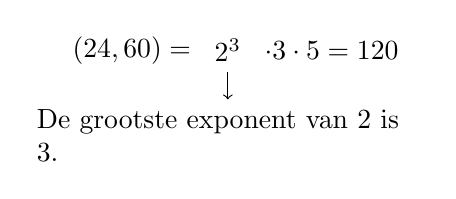
\begin{tikzpicture}
\node (a) {$\kgv(24,60)=$};
\node (b) [right=0.15em of a] {$2^3$};
\node (c) [right=0.15em of b] {$\cdot3\cdot5=120$};
\draw[->] (b.south) -- ++(0,-1em)
  node[below,text width=0.4\textwidth,align=left] {De grootste exponent van 2 is 3.};
\end{tikzpicture}
\end{center}
\end{voorbeeld}

\begin{voorbeeld}
$\kgv(130,195,225)=?$
\[\priemontbind[v]{130}\qquad\qquad\priemontbind[v]{195}\qquad\qquad\priemontbind[v]{225}\]
\[\kgv(130,195,225)=2\cdot3^2\cdot5^2\cdot13=5\,850\]
\end{voorbeeld}

\subsubsection{Grootste gemene deler}

De gemeenschappelijke delers van 12 en 8 zijn $1,2$ en 4. De \textbf{grootste gemene (of
gemeenschappelijke) deler} (g.g.d.) is 4.

Om de grootste gemene deler te bepalen van 2 niet te grote getallen, som je van elk getal de
delers op. Om de g.g.d. te bepalen van grotere getallen gebruik je volgende werkwijze:

\begin{voorbeeld}
$\ggd(24,60)=?$
\begin{itemize}
  \item ontbind in priemfactoren
  \item maak het product van de \emph{gemeenschappelijke} priemfactoren, elk met de
  \emph{kleinste} exponent
\end{itemize}
\[\priemontbind[h]{24}\qquad\qquad\priemontbind[h]{60}\]
\[\qquad\qquad\qquad\ggd(24,60)=2^2\cdot3=12\qquad\text{(5 is niet gemeenschappelijk)}\]
\end{voorbeeld}

\begin{voorbeeld}
$\ggd(130,195,225)=?$ (voor de ontbinding, zie k.g.v.)
\[\priemfactorisatie{130}\qquad\priemfactorisatie{195}\qquad\priemfactorisatie{225}\]
\[\ggd(130,195,225)=5\]
\end{voorbeeld}

\begin{voorbeeld}
$\ggd(26,35)=?$
\[\priemfactorisatie{26}\qquad\priemfactorisatie{35}\]
\[\ggd(26,35)=1\]
Als de grootste gemene deler van enkele getallen gelijk is aan 1, dan zijn deze getallen
\textbf{onderling ondeelbaar}.
\end{voorbeeld}

\begin{exercise}
Kruis het juiste antwoord aan: 9 is een gemene deler van:
\begin{meerkeuze}
  \item 9 en 39
  \item 49 en 99
  \item 54 en 84
  \item 27 en 63
\end{meerkeuze}
\end{exercise}

\begin{solution}
\textbf{Antwoord (D)} is juist.
\end{solution}

\begin{exercise}
Zoek alle getallen kleiner dan 10, die onderling ondeelbaar zijn met 8.
\end{exercise}

\begin{solution}
Onderling ondeelbaar met 8 zijn: 1 en 8; 3 en 8; 5 en 8; 7 en 8; 9 en 8.
\end{solution}

\begin{exercise}
Bereken de g.g.d. en k.g.v. van:
\begin{enumerate}
  \item 112 en 84
  \item 432, 648 en 792
\end{enumerate}
\end{exercise}

\begin{solution}
\begin{enumerate}
  \item $\priemontbind[v]{112}\qquad\priemontbind[v]{84}$\\
  $\ggd(112,84)=2^2\cdot7=28\qquad\kgv(112,84)=2^4\cdot3\cdot7=336$
  \item $\priemontbind[v]{432}\qquad\priemontbind[v]{648}\qquad\priemontbind[v]{792}$\\
  $\ggd(432,648,792)=2^3\cdot3^2=72\qquad\kgv(432,648,792)=2^4\cdot3^4\cdot11=14\,256$
\end{enumerate}
\end{solution}

\pagebreak
\begin{mdframed}
  \subsection*{Samenvatting}

  Als men bij beide leden van een gelijkheid eenzelfde getal optelt, aftrekt of beide leden
  vermenigvuldigt met of deelt door eenzelfde getal, bekomt men een nieuwe gelijkheid.

  Als men bij beide leden van een ongelijkheid eenzelfde getal optelt of aftrekt, bekomt men een
  nieuwe ongelijkheid in dezelfde zin. Vermenigvuldigt of deelt men beide leden met eenzelfde
  \emph{strikt positief} getal, dan blijft de ongelijkheid in dezelfde zin; met een \emph{strikt
    negatief} getal draait ze om.

  Als men 2 gelijkheden lid aan lid optelt, aftrekt, vermenigvuldigt of deelt, bekomt men een
  nieuwe gelijkheid.

  Als men 2 ongelijkheden in dezelfde zin lid aan lid optelt of vermenigvuldigt, bekomt men een
  nieuwe ongelijkheid in dezelfde zin.

  \textbf{Transitieve eigenschap:}
  \begin{align*}
    a=b\text{ en }b=c&\quad\Rightarrow\quad a=c\\
    a<b\text{ en }b<c&\quad\Rightarrow\quad a<c
  \end{align*}

  \textbf{Kenmerken van deelbaarheid}
  \begin{itemize}
  \item door 2, 5, 10: laatste cijfer deelbaar door 2, 5, 10
  \item door 4, 25, 100: laatste 2 cijfers deelbaar door 4, 25, 100
  \item door 8, 125, 1\,000: laatste 3 cijfers deelbaar door 8, 125, 1\,000
  \item door 3, 9: som der cijfers deelbaar door 3 of 9
  \item door 11: som van de cijfers van oneven rang min som van de cijfers van even rang
    deelbaar door 11
  \end{itemize}
\end{mdframed}

\oplossingen

\end{document}
